%
% p4_hw6.tex
%
% 05Aug17  Jackson Sheppard
%
\documentclass[12pt]{article}
\usepackage{fancyhdr}
\usepackage{graphicx}
\usepackage{color}
\usepackage{hyperref}
\usepackage{indentfirst}

% Uncomment one of the following lines to use Times-Roman and Helvetica
% or Palatino instead of Computer Modern.
% \usepackage{txfonts}
% \usepackage[sc]{mathpazo}\linespread{1.05}\usepackage[scaled]{helvet}

\usepackage[hmargin=90bp,tmargin=108bp,bmargin=72bp,
            headheight=15bp,footskip=40bp]{geometry}
%%%%%%%%%%%%%%%%%%%%%%%%%%%%%%%%%%%%%%%%%%%%%%%%%%%%%%%%%%%%%%%%%%%%%%%%%%%%%%%

%
% custom definitions
%
\newcommand\thisis{Problem 4: Coin Toss Simulation}
\newcommand\theauthor{Jackson~Sheppard}

\newcommand\sfb{\sffamily\bfseries}

\newcommand\red[1]{\textcolor{red}{\sffamily\bfseries #1}}
%%%%%%%%%%%%%%%%%%%%%%%%%%%%%%%%%%%%%%%%%%%%%%%%%%%%%%%%%%%%%%%%%%%%%%%%%%%%%%%

%
% custom heading and footer
%
\fancypagestyle{firstpg}
   {
   \fancyhf{}%
   \cfoot{\sffamily\thepage}%
   \renewcommand\headrulewidth{0bp}
   }

\pagestyle{fancy}
\lhead{\sffamily \thisis}
\chead{}
\rhead{\sffamily \theauthor}

\lfoot{}
\cfoot{\sffamily\thepage}
\rfoot{}
%%%%%%%%%%%%%%%%%%%%%%%%%%%%%%%%%%%%%%%%%%%%%%%%%%%%%%%%%%%%%%%%%%%%%%%%%%%%%%%

\begin{document}
\thispagestyle{firstpg}

\noindent
{\sffamily\bfseries\huge \thisis}\\

\noindent
{\large\sffamily \theauthor}

\vspace*{20bp}


The program "p4\_hw5.py" contains a function simulating $100$ coin tosses and
returns the number of heads thrown. It then plots a histogram displaying the
result of calling the functuin $1000$ times and each time recording the number
of heads returned. The program then overlays on the plot a graph of the Gaussian
distribution with the same mean and standard deviation as the binomial
distribution that corresponds to the coin toss simulation.

The function simulating $100$ coin tosses is called "coin\_toss". It simulates
the process by initializing a count variable to zero and then choosing a random
integer between zero and one using the numpy function "randint". Assigning zero
to heads and one to tails, the program repeats this process $100$ times, adding
one to the count variable each time a zero is chosen, and then returns the
count.

The program then plots the histogram displaying the result of 1000 function
calls by initializing an array "num\_heads" with $1000$ entries and then
iterating through each entry and storing the result of the function call.
It then plots the histogram (shown in blue in Fig.~\ref{fig:hist}) displaying
on the horizontal axis the number of heads returned and on the vertical axis the
total number of occurances in $1000$ function calls of that range of numbers of
successes. In order to effectively overlay the Gaussian distribution onto this
plot, we specify to plot a normalized histogram which instead divides each total
number of occurances by the total number of function calls.

%------------------------------------------------------------------------------
\begin{figure}[h]
\begin{center}
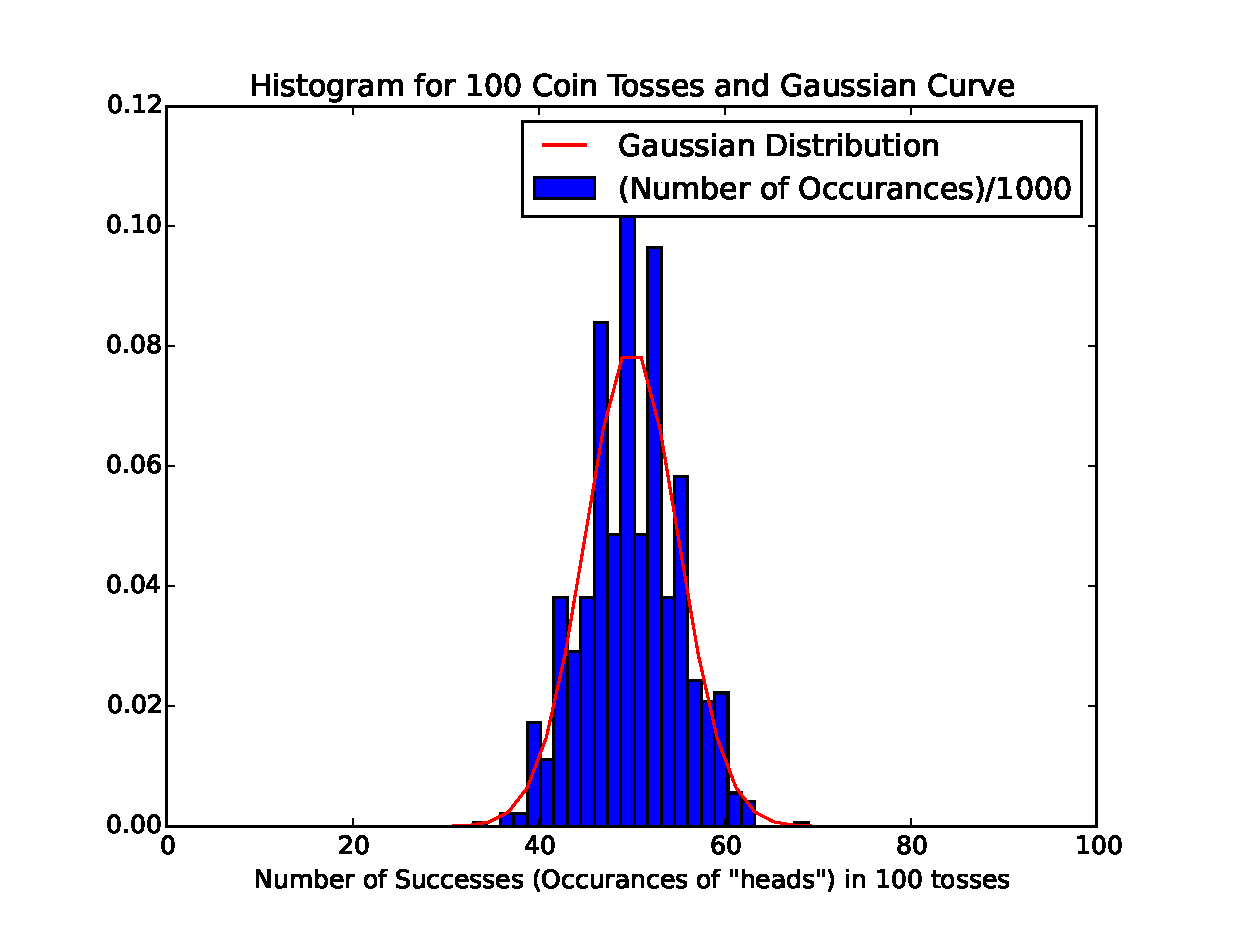
\includegraphics[width=300bp]{p4_hw6_histgauss.eps}
\vspace{-18bp}
\end{center}
\caption[]{\label{fig:hist}\small
In blue, we have the normalized histogram for the result of $1000$ total
function calls to the function "coin\_toss" which returns the number of "heads"
in $100$ coin tosses. The horizontal axis contains the number of possible
"heads" achieved for any given simulation, while the vertical axis is normalized
to contain the ratio of the number of occurances of each range of numbers of
successes to the total number of function calls, $1000$. In red, we have the
Gaussian distribution with the same mean and standard deviation of this simulation.
}
\end{figure}
%------------------------------------------------------------------------------

After plotting the normalized histogram, the program overlays on the plot a
graph of the Gaussian distribution with same mean and standard deviation as
this simulation. The result is shown in red in Fig.~\ref{fig:hist}.
The gaussian distribution is defined as follows:
\begin{equation} \label{eq:1}
G(x) = \frac{1}{\sigma\sqrt{2\pi}}e^{-(x-\mu)^2/2\sigma^2}
\end{equation}

Here $\mu=Np$ is the mean and $\sigma=\sqrt{Npq}$ is the standard deviation.
In these definitions, $N$ is the number of attempts, in this case $100$, $p$ is the probability of success, in this case $0.5$, and $q=1-p$ is the probability
of failure. The program then simply calculates the mean and standard deviation
for this simulation and plots $G(x)$ over the range of $x=0$ to $x=100$
coinciding with the possible numbers of successes in this simulation. We see
from the plot in Fig.~\ref{fig:hist} that the Gaussian distribution well
approximates the binomial distribution of this simulation.

\end{document}

